%% bare_jrnl_compsoc.tex
%% V1.4b
%% 2015/08/26
%% by Michael Shell
%% See:
%% http://www.michaelshell.org/
%% for current contact information.
%%
%% This is a skeleton file demonstrating the use of IEEEtran.cls
%% (requires IEEEtran.cls version 1.8b or later) with an IEEE
%% Computer Society journal paper.
%%
%% Support sites:
%% http://www.michaelshell.org/tex/ieeetran/
%% http://www.ctan.org/pkg/ieeetran
%% and
%% http://www.ieee.org/

%%*************************************************************************
%% Legal Notice:
%% This code is offered as-is without any warranty either expressed or
%% implied; without even the implied warranty of MERCHANTABILITY or
%% FITNESS FOR A PARTICULAR PURPOSE! 
%% User assumes all risk.
%% In no event shall the IEEE or any contributor to this code be liable for
%% any damages or losses, including, but not limited to, incidental,
%% consequential, or any other damages, resulting from the use or misuse
%% of any information contained here.
%%
%% All comments are the opinions of their respective authors and are not
%% necessarily endorsed by the IEEE.
%%
%% This work is distributed under the LaTeX Project Public License (LPPL)
%% ( http://www.latex-project.org/ ) version 1.3, and may be freely used,
%% distributed and modified. A copy of the LPPL, version 1.3, is included
%% in the base LaTeX documentation of all distributions of LaTeX released
%% 2003/12/01 or later.
%% Retain all contribution notices and credits.
%% ** Modified files should be clearly indicated as such, including  **
%% ** renaming them and changing author support contact information. **
%%*************************************************************************


% *** Authors should verify (and, if needed, correct) their LaTeX system  ***
% *** with the testflow diagnostic prior to trusting their LaTeX platform ***
% *** with production work. The IEEE's font choices and paper sizes can   ***
% *** trigger bugs that do not appear when using other class files.       *** 
% The testflow support page is at:                                        ***
% http://www.michaelshell.org/tex/testflow/


\documentclass[10pt,journal,compsoc]{IEEEtran}

% *** CITATION PACKAGES ***
%
\ifCLASSOPTIONcompsoc
% IEEE Computer Society needs nocompress option
% requires cite.sty v4.0 or later (November 2003)
\usepackage[nocompress]{cite}
\else
% normal IEEE
\usepackage{cite}
\fi
% cite.sty was written by Donald Arseneau
% V1.6 and later of IEEEtran pre-defines the format of the cite.sty package
% \cite{} output to follow that of the IEEE. Loading the cite package will
% result in citation numbers being automatically sorted and properly
% "compressed/ranged". e.g., [1], [9], [2], [7], [5], [6] without using
% cite.sty will become [1], [2], [5]--[7], [9] using cite.sty. cite.sty's
% \cite will automatically add leading space, if needed. Use cite.sty's
% noadjust option (cite.sty V3.8 and later) if you want to turn this off
% such as if a citation ever needs to be enclosed in parenthesis.
% cite.sty is already installed on most LaTeX systems. Be sure and use
% version 5.0 (2009-03-20) and later if using hyperref.sty.
% The latest version can be obtained at:
% http://www.ctan.org/pkg/cite
% The documentation is contained in the cite.sty file itself.
%
% Note that some packages require special options to format as the Computer
% Society requires. In particular, Computer Society  papers do not use
% compressed citation ranges as is done in typical IEEE papers
% (e.g., [1]-[4]). Instead, they list every citation separately in order
% (e.g., [1], [2], [3], [4]). To get the latter we need to load the cite
% package with the nocompress option which is supported by cite.sty v4.0
% and later. Note also the use of a CLASSOPTION conditional provided by
% IEEEtran.cls V1.7 and later.





% *** GRAPHICS RELATED PACKAGES ***
%
\ifCLASSINFOpdf
\usepackage{graphicx}
% declare the path(s) where your graphic files are
\graphicspath{{Figures/}{Other_Folder/}}
% and their extensions so you won't have to specify these with
% every instance of \includegraphics
\DeclareGraphicsExtensions{.pdf,.jpeg,.png}
\else
% or other class option (dvipsone, dvipdf, if not using dvips). graphicx
% will default to the driver specified in the system graphics.cfg if no
% driver is specified.
% \usepackage[dvips]{graphicx}
% declare the path(s) where your graphic files are
% \graphicspath{{../eps/}}
% and their extensions so you won't have to specify these with
% every instance of \includegraphics
% \DeclareGraphicsExtensions{.eps}
\fi
% graphicx was written by David Carlisle and Sebastian Rahtz. It is
% required if you want graphics, photos, etc. graphicx.sty is already
% installed on most LaTeX systems. The latest version and documentation
% can be obtained at: 
% http://www.ctan.org/pkg/graphicx
% Another good source of documentation is "Using Imported Graphics in
% LaTeX2e" by Keith Reckdahl which can be found at:
% http://www.ctan.org/pkg/epslatex
%
% latex, and pdflatex in dvi mode, support graphics in encapsulated
% postscript (.eps) format. pdflatex in pdf mode supports graphics
% in .pdf, .jpeg, .png and .mps (metapost) formats. Users should ensure
% that all non-photo figures use a vector format (.eps, .pdf, .mps) and
% not a bitmapped formats (.jpeg, .png). The IEEE frowns on bitmapped formats
% which can result in "jaggedy"/blurry rendering of lines and letters as
% well as large increases in file sizes.
%
% You can find documentation about the pdfTeX application at:
% http://www.tug.org/applications/pdftex






% *** MATH PACKAGES ***
%
%\usepackage{amsmath}
% A popular package from the American Mathematical Society that provides
% many useful and powerful commands for dealing with mathematics.
%
% Note that the amsmath package sets \interdisplaylinepenalty to 10000
% thus preventing page breaks from occurring within multiline equations. Use:
%\interdisplaylinepenalty=2500
% after loading amsmath to restore such page breaks as IEEEtran.cls normally
% does. amsmath.sty is already installed on most LaTeX systems. The latest
% version and documentation can be obtained at:
% http://www.ctan.org/pkg/amsmath


% *** SUBFIGURE PACKAGES ***
\ifCLASSOPTIONcompsoc
\usepackage[caption=false,font=footnotesize,labelfont=sf,textfont=sf]{subfig}
\else
\usepackage[caption=false,font=footnotesize]{subfig}
\fi
% subfig.sty, written by Steven Douglas Cochran, is the modern replacement
% for subfigure.sty, the latter of which is no longer maintained and is
% incompatible with some LaTeX packages including fixltx2e. However,
% subfig.sty requires and automatically loads Axel Sommerfeldt's caption.sty
% which will override IEEEtran.cls' handling of captions and this will result
% in non-IEEE style figure/table captions. To prevent this problem, be sure
% and invoke subfig.sty's "caption=false" package option (available since
% subfig.sty version 1.3, 2005/06/28) as this is will preserve IEEEtran.cls
% handling of captions.
% Note that the Computer Society format requires a sans serif font rather
% than the serif font used in traditional IEEE formatting and thus the need
% to invoke different subfig.sty package options depending on whether
% compsoc mode has been enabled.
%
% The latest version and documentation of subfig.sty can be obtained at:
% http://www.ctan.org/pkg/subfig


% *** PDF, URL AND HYPERLINK PACKAGES ***
%
\usepackage{url}
\usepackage{hyperref}
% url.sty was written by Donald Arseneau. It provides better support for
% handling and breaking URLs. url.sty is already installed on most LaTeX
% systems. The latest version and documentation can be obtained at:
% http://www.ctan.org/pkg/url
% Basically, \url{my_url_here}.

% correct bad hyphenation here
\hyphenation{}

\begin{document}
	
	
	\title{BGWS: A Dependable Decentralized Ledger for a
	Blockchained Global Wallet Service}
	% author names and IEEE memberships
	% note positions of commas and nonbreaking spaces ( ~ ) LaTeX will not break
	% a structure at a ~ so this keeps an author's name from being broken across
	% two lines.
	% use \thanks{} to gain access to the first footnote area
	% a separate \thanks must be used for each paragraph as LaTeX2e's \thanks
	% was not built to handle multiple paragraphs
	%
	%
	%\IEEEcompsocitemizethanks is a special \thanks that produces the bulleted
	% lists the Computer Society journals use for "first footnote" author
	% affiliations. Use \IEEEcompsocthanksitem which works much like \item
	% for each affiliation group. When not in compsoc mode,
	% \IEEEcompsocitemizethanks becomes like \thanks and
	% \IEEEcompsocthanksitem becomes a line break with idention. This
	% facilitates dual compilation, although admittedly the differences in the
	% desired content of \author between the different types of papers makes a
	% one-size-fits-all approach a daunting prospect. For instance, compsoc 
	% journal papers have the author affiliations above the "Manuscript
	% received ..."  text while in non-compsoc journals this is reversed. Sigh.
		\author{Diogo Cebola, 52718 and \and
		Gonçalo Areia, 52714}% <-this % stops a space

	%\IEEEtitleabstractindextext{
		
		

	%}
	
	
	\maketitle
	% To allow for easy dual compilation without having to reenter the
	% abstract/keywords data, the \IEEEtitleabstractindextext text will
	% not be used in maketitle, but will appear (i.e., to be "transported")
	% here as \IEEEdisplaynontitleabstractindextext when the compsoc 
	% or transmag modes are not selected <OR> if conference mode is selected 
	% - because all conference papers position the abstract like regular
	% papers do.
	\IEEEdisplaynontitleabstractindextext
	% \IEEEdisplaynontitleabstractindextext has no effect when using
	% compsoc or transmag under a non-conference mode.
	
	% For peer review papers, you can put extra information on the cover
	% page as needed:
	% \ifCLASSOPTIONpeerreview
	% \begin{center} \bfseries EDICS Category: 3-BBND \end{center}
	% \fi
	%
	% For peerreview papers, this IEEEtran command inserts a page break and
	% creates the second title. It will be ignored for other modes.

	%\IEEEpeerreviewmaketitle
	\begin{abstract}
		
	\end{abstract}


	\begin{IEEEkeywords}
			
	\end{IEEEkeywords}

	%\vspace{\line}
	%\IEEEraisesectionheading{\label{sec:introduction}}
	\section{Introduction}

	%(defining the problem, goals/objectives and initial presentation of the solution as a way to address the problem). Finish this with a summary of the organization of the remaining

	\IEEEPARstart{T}{}his work was proposed by professor Henrique Domingos as the course project of “Dependable Distributed Systems“ 2020-21.
	Since the appearance 
		
	The remaining of the document is organized as follows.
	In Section 2, we introduce important concepts related to our work, more specifically Byzantine Fault Tolerance and the Blockchain technology.
	In Section 3, we present BGWS system model and architecture.
	Internal mechanisms, design assumptions and the service planes are covered in section 4.
	In Section 5, we explain implementation details (e.g. technologies used and development issues).
	Section 4 will present the experimental setting and discuss the obtained results.
	Finally, in Section 5 we conclude the document and mention future work.\cite{nakamoto2019bitcoin}
	



	\section{Background}
	\subsection{Byzantine Fault Tolerance}
	\subsection{Blockchain Technology}
	\section{System Model and Architecture}

	% Present the system model and then the architecture of your solution ? Try to clarify the reader to understand the main APIs and interfaces in your solution and the role of the components in the architecture in a structured way 

	\section{Mechanisms and Service Planes}

	% Can explain in more detail the internals of the more relevant components and their highlights, in the way you decide to design and implement and why. System design assumptions, principles, paradigms, concepts and abstractions and fundamental techniques.

	\section{Implementation}
	\subsection{Technology Stack}
	\subsection{Issues}

	
	\section{Experimental Evaluation}
	\subsection{Experimental Setup \& Methodology}
	\subsubsection{Validation}
	\subsubsection{Evaluation}
	\subsection{Experimental Results}
	
	In this section we present the results as an average of the three runs executed, and describe the patterns observed.
	
	%\begin{figure}[!ht]
	%	\centering
	%	\subfloat[Default workload test]{
%			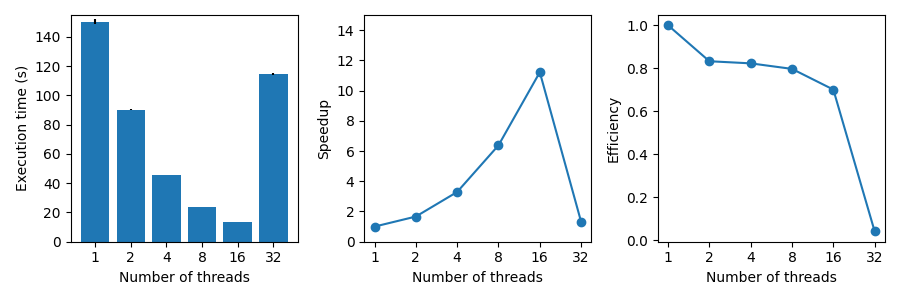
\includegraphics[width=\linewidth]{figures/test_02.png}
%			\label{default_workload_test}
%		}
%		\vfil
%		\subfloat[Uniform workload test.]{
%			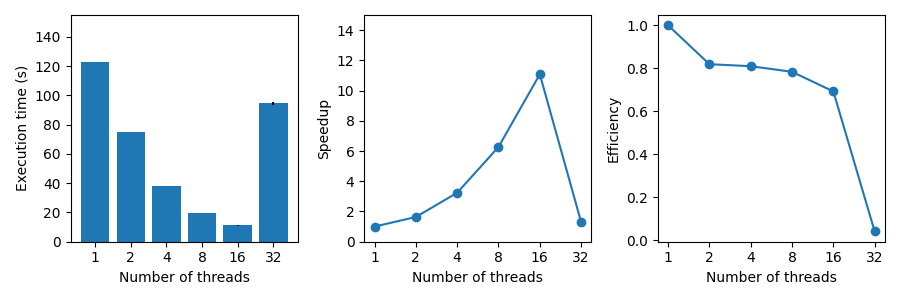
\includegraphics[width=\linewidth]{figures/test_11.png}
%			\label{uniform_workload_test}
%		}
%		\vfil
%		\centering
%		\subfloat[Triangular workload test.]{
%			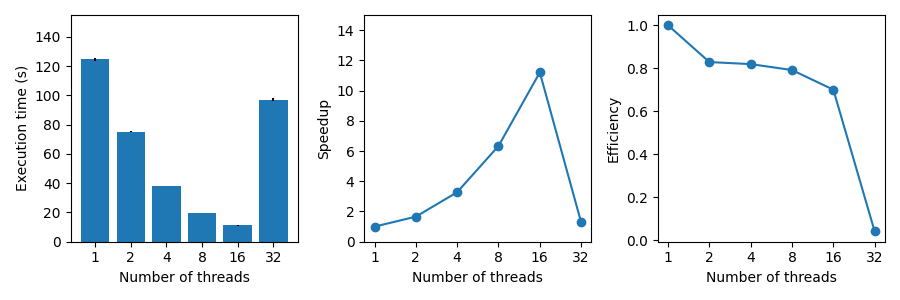
\includegraphics[width=\linewidth]{figures/test_13.png}
%			\label{triangular_workload_test}
%		}
%		\vfil
%		\subfloat[Reduction efficiency test.]{
%			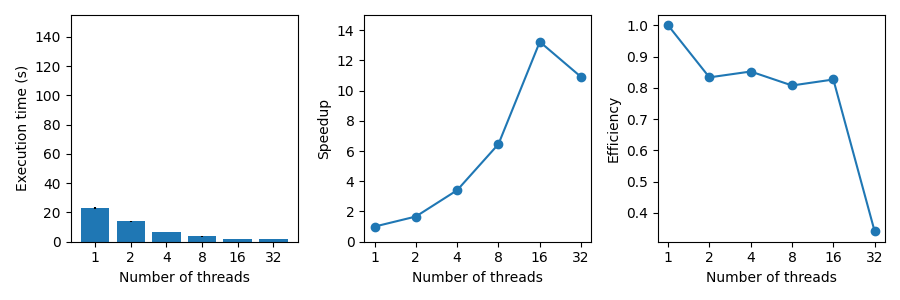
\includegraphics[width=\linewidth]{figures/test_08.png}
%			\label{reduction_efficiency_test}
%		}
%		\caption{Execution time, speedup and efficiency.}
%	\end{figure}
	
	\subsection{Discussion}
	In this section we will discuss the variation in the results obtained for the different experiments.
	
	\section{Coverage of Requirements}
	% Coverage of the requirements (Summarize here the coverage (emphasining the completness, correctness, drawbacks, limitations or tradeofs) form the expected requirements.

	\section{Conclusion \& Future Work}

	\ifCLASSOPTIONcaptionsoff
	\newpage
	\fi
	\nocite{*}
	\bibliographystyle{IEEEtran}
	\bibliography{references}
	
\end{document}
